\section{Test Description and Success Criteria}
This test is located in \texttt{simulation/dynamics/FuelTank/UnitTest/\newline
test\_fuelSloshParticleStateEffector.py}. In this integrated test there are three fuel slosh particles connected to the spacecraft hub.  Depending on the scenario, there are different success criteria. These are outlined in the following subsections:
\subsection{Gravity integrated test}
In this test the simulation is placed into orbit around Earth with point gravity and has no damping in the fuel slosh particles. The following parameters are being tested. 
\begin{itemize}
	\item Conservation of orbital angular momentum
	\item Conservation of orbital energy
	\item Conservation of rotational angular momentum
	\item Conservation of rotational energy
\end{itemize}

\subsection{No gravity integrated test}
In this test, the spacecraft is placed in free space (no gravity) and has no damping in the fuel slosh particles. The following parameters describe the success criteria.
\begin{itemize}
\item Conservation of orbital angular momentum
\item Conservation of orbital energy
\item Conservation of rotational angular momentum
\item Conservation of rotational energy
\end{itemize}

\subsection{Damping with no gravity integrated test}
In this test, the spacecraft is placed in free space (no gravity) and has damping in the fuel slosh particles. The following parameters describe the success criteria.
\begin{itemize}
	\item Conservation of orbital angular momentum
	\item Conservation of orbital energy
	\item Conservation of rotational angular momentum
\end{itemize}

\section{Test Parameters}

Since this is an integrated test, the inputs to the test are the physical parameters of the spacecraft along with the initial conditions of the states. These parameters are outlined in Tables~\ref{tab:hub}-~\ref{tab:initial}. Additionally, the error tolerances can be seen in Table~\ref{tab:errortol}. The error tolerance for the energy and momentum tests is 1e-10 and that was chosen to ensure cross platform success of the test, however it is expected to get conservation of energy and momentum down to 1e-14 or lower. 

\begin{table}[htbp]
	\caption{Spacecraft Hub Parameters}
	\label{tab:hub}
	\centering \fontsize{10}{10}\selectfont
	\begin{tabular}{| c | c | c | c |} % Column formatting, 
		\hline
		\textbf{Name}  & \textbf{Description}  & \textbf{Value} & \textbf{Units} \\
		\hline
		mHub  & mass & 750.0 & kg \\
		\hline
		IHubPntBc\_B & Inertia in $\cal{B}$ frame & $\begin{bmatrix}
		900.0 & 0.0 & 0.0\\
		0.0 & 600.0 & 0.0\\
		0.0 & 0.0 & 600.0
		\end{bmatrix}$ & kg-m$^2$ \\
		\hline
		r\_BcB\_B & CoM Location in $\cal{B}$ frame & $\begin{bmatrix}
		0.0 & 0.0 & 0.0 \end{bmatrix}^T$ & m \\
		\hline
	\end{tabular}
\end{table}

\begin{table}[htbp]
	\caption{Fuel Slosh Particle 1 Parameters}
	\label{tab:slosh1}
	\centering \fontsize{10}{10}\selectfont
	\begin{tabular}{| c | c | c | c |} % Column formatting, 
		\hline
		\textbf{Name}  & \textbf{Description}  & \textbf{Value} & \textbf{Units} \\
		\hline
		mass  & mass & 10.0 & kg \\
		\hline
		k & Spring Constant & 100.0 & N-m/rad \\
		\hline
		c & Damping Term & 0.0 (15.0 for Damping Case) & N-m-s/rad \\
		\hline
		r\_PB\_B & Slosh Equilibrium Location in $\cal{B}$ frame & $\begin{bmatrix}
		0.1 & 0.0 & -0.1 \end{bmatrix}^T$ & m \\
		\hline
		pHat\_B & Slosh direction in $\cal{B}$ frame & $\begin{bmatrix}
		\frac{\sqrt{3}}{3} & \frac{\sqrt{3}}{3} & \frac{\sqrt{3}}{3} \end{bmatrix}^T$ & 1 \\
		\hline
	\end{tabular}
\end{table}

\begin{table}[htbp]
	\caption{Fuel Slosh Particle 2 Parameters}
	\label{tab:slosh2}
	\centering \fontsize{10}{10}\selectfont
	\begin{tabular}{| c | c | c | c |} % Column formatting, 
		\hline
		\textbf{Name}  & \textbf{Description}  & \textbf{Value} & \textbf{Units} \\
		\hline
		mass  & mass & 10.0 & kg \\
		\hline
		k & Spring Constant & 100.0 & N-m/rad \\
		\hline
		c & Damping Term & 0.0 (17.0 for Damping Case) & N-m-s/rad \\
		\hline
		r\_PB\_B & Slosh Equilibrium Location in $\cal{B}$ frame & $\begin{bmatrix}
		0.0 & 0.0 & 0.1 \end{bmatrix}^T$ & m \\
		\hline
		pHat\_B & Slosh direction in $\cal{B}$ frame & $\begin{bmatrix}
		\frac{\sqrt{3}}{3} & -\frac{\sqrt{3}}{3} & -\frac{\sqrt{3}}{3} \end{bmatrix}^T$ & 1 \\
		\hline
	\end{tabular}
\end{table}

\begin{table}[htbp]
	\caption{Fuel Slosh Particle 3 Parameters}
	\label{tab:slosh3}
	\centering \fontsize{10}{10}\selectfont
	\begin{tabular}{| c | c | c | c |} % Column formatting, 
		\hline
		\textbf{Name}  & \textbf{Description}  & \textbf{Value} & \textbf{Units} \\
		\hline
		mass  & mass & 10.0 & kg \\
		\hline
		k & Spring Constant & 100.0 & N-m/rad \\
		\hline
		c & Damping Term & 0.0 (11.0 for Damping Case) & N-m-s/rad \\
		\hline
		r\_PB\_B & Slosh Equilibrium Location in $\cal{B}$ frame & $\begin{bmatrix}
		-0.1 & 0.0 & 0.1 \end{bmatrix}^T$ & m \\
		\hline
		pHat\_B & Slosh direction in $\cal{B}$ frame & $\begin{bmatrix}
		-\frac{\sqrt{3}}{3} & -\frac{\sqrt{3}}{3} & \frac{\sqrt{3}}{3} \end{bmatrix}^T$ & 1 \\
		\hline
	\end{tabular}
\end{table}

\begin{table}[htbp]
	\caption{Initial Conditions}
	\label{tab:initial}
	\centering \fontsize{10}{10}\selectfont
	\begin{tabular}{| c | c | c | c |} % Column formatting, 
		\hline
		\textbf{Name}  & \textbf{Description}  & \textbf{Value} & \textbf{Units} \\
		\hline
		(Particle 1) rhoInit  & (Particle 1) Initial $\rho$ & 0.05 & m \\
		\hline
		(Particle 1) rhoDotInit  & (Particle 1) Initial $\dot{\rho}$ & 0.0 & m/s \\
		\hline
		(Particle 2) rhoInit  & (Particle 2) Initial $\rho$ & -0.025 & m \\
		\hline
		(Particle 2) rhoDotInit  & (Particle 2) Initial $\dot{\rho}$ & 0.0 & m/s \\
		\hline
		(Particle 3) rhoInit  & (Particle 3) Initial $\rho$ & -0.015 & m \\
		\hline
		(Particle 3) rhoDotInit  & (Particle 3) Initial $\dot{\rho}$ & 0.0 & m/s \\
		\hline
		r\_CN\_NInit & Initial Position of S/C (gravity scenarios) & $\begin{bmatrix}
		-4020339 &	7490567 & 5248299 
		\end{bmatrix}^T$ & m \\
		\hline
		v\_CN\_NInit & Initial Velocity of S/C (gravity scenarios) & $\begin{bmatrix}
		-5199.78 & -3436.68 & 1041.58
		\end{bmatrix}^T$ & m/s \\
		\hline
		r\_CN\_NInit & Initial Position of S/C (no gravity) & $\begin{bmatrix}
		0.5 & 0.4 & -0.7 
		\end{bmatrix}^T$ & m \\
		\hline
		v\_CN\_NInit & Initial Velocity of S/C (no gravity) & $\begin{bmatrix}
		0.1 & -0.5 & 0.3
		\end{bmatrix}^T$ & m/s \\
		\hline
		sigma\_BNInit & Initial MRP of $\cal{B}$ frame & $\begin{bmatrix}
		0.0 & 0.0 & 0.0
		\end{bmatrix}^T$ & 1 \\
		\hline
		omega\_BN\_BInit & Initial Angular Velocity of $\cal{B}$ frame & $\begin{bmatrix}
		0.1 & -0.1 & 0.1
		\end{bmatrix}^T$ & rad/s \\
		\hline
	\end{tabular}
\end{table}

\begin{table}[htbp]
	\caption{Error Tolerance - Note: Relative Tolerance is $\textnormal{abs}(\frac{\textnormal{truth} - \textnormal{value}}{\textnormal{truth}}$)}
	\label{tab:errortol}
	\centering \fontsize{10}{10}\selectfont
	\begin{tabular}{| c | c |} % Column formatting, 
		\hline
		Test   & Relative Tolerance \\
		\hline
		Energy and Momentum Conservation & 1e-10 \\
		\hline	
	\end{tabular}
\end{table}

\clearpage

\section{Test Results}

The following figures show the conservation of the quantities described in the success criteria for each scenario. The conservation plots are all relative difference plots. All conservation plots show integration error which is the desired result. In the python test these values are automatically checked therefore when the tests pass, these values have all been confirmed to be conserved. An additional note: the angular momentum plots are plotting the change in the components of the angular momentum vector in the inertial frame. The individual components are not labeled because the goal is for each component to show conservation therefore the individual components do not have separate information needing to be specified.  

\subsection{Gravity with no damping scenario}
\begin{figure}[htbp]
	\centerline{
		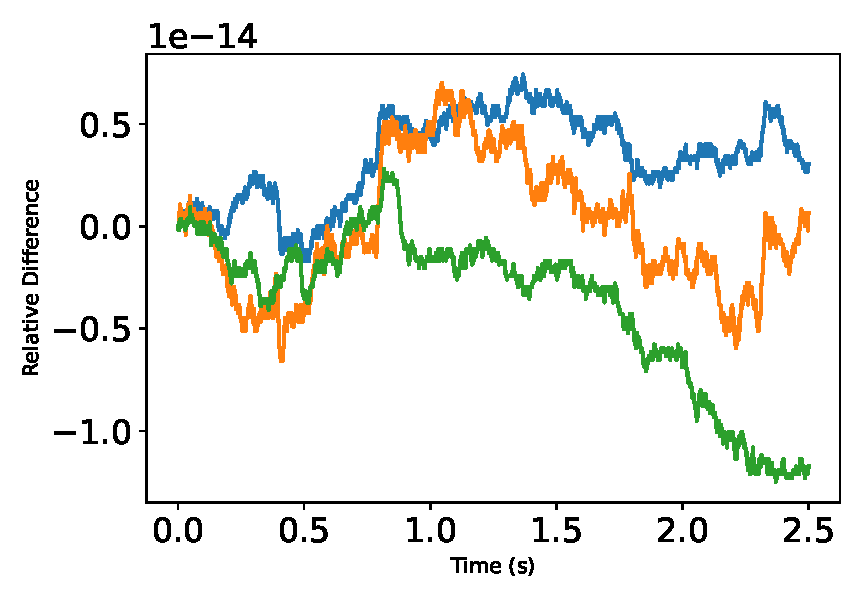
\includegraphics[width=0.8\textwidth]{AutoTeX/ChangeInOrbitalAngularMomentumGravity}}
	\caption{Change in Orbital Angular Momentum Gravity}
	\label{fig:ChangeInOrbitalAngularMomentumGravity}
\end{figure}
\begin{figure}[htbp]
	\centerline{
		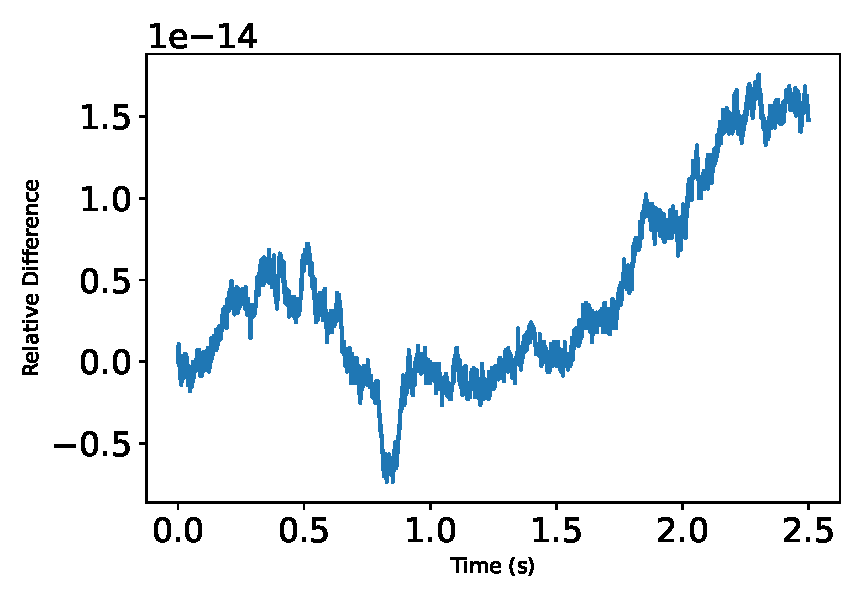
\includegraphics[width=0.8\textwidth]{AutoTeX/ChangeInOrbitalEnergyGravity}}
	\caption{Change in Orbital Energy Gravity}
	\label{fig:ChangeInOrbitalEnergyGravity}
\end{figure}
\begin{figure}[htbp]
	\centerline{
		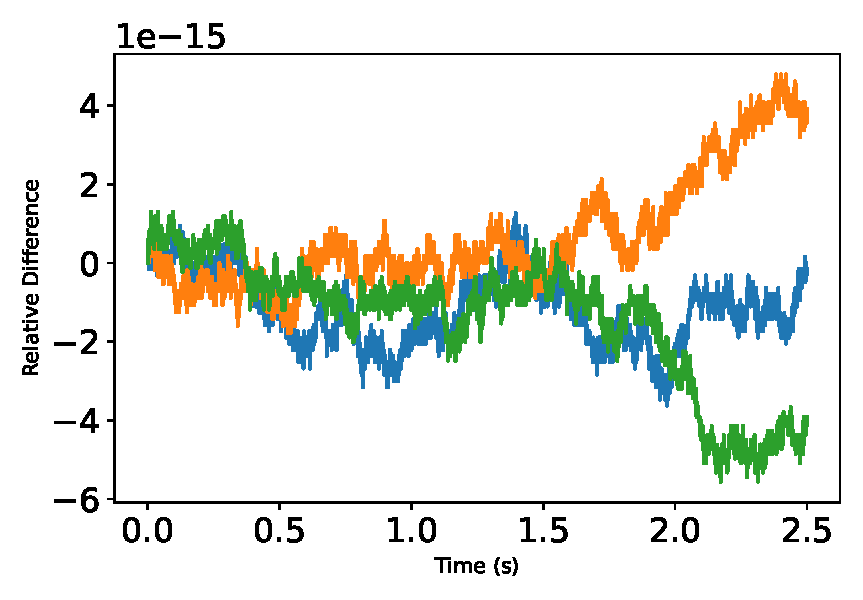
\includegraphics[width=0.8\textwidth]{AutoTeX/ChangeInRotationalAngularMomentumGravity}}
	\caption{Change In Rotational Angular Momentum Gravity}
	\label{fig:ChangeInRotationalAngularMomentumGravity}
\end{figure}
\begin{figure}[htbp]
	\centerline{
		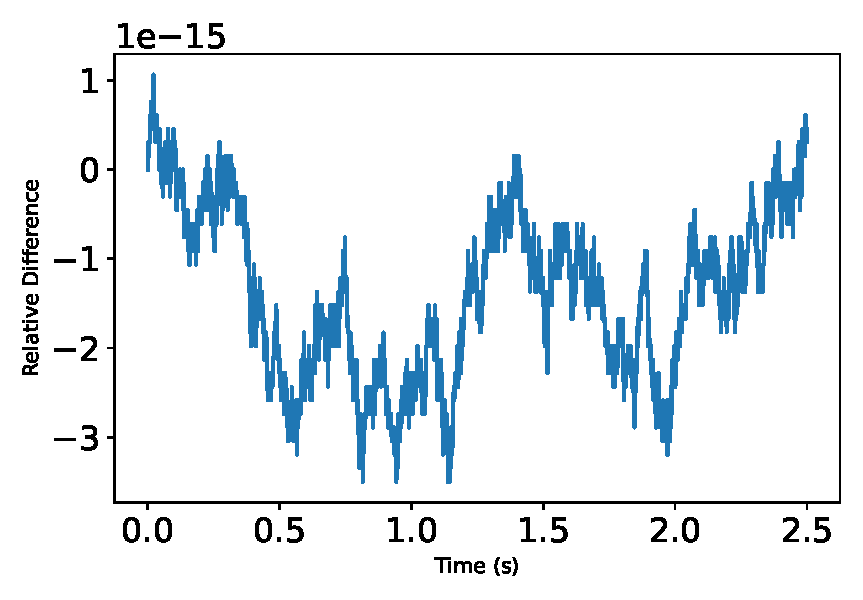
\includegraphics[width=0.8\textwidth]{AutoTeX/ChangeInRotationalEnergyGravity}}
	\caption{Change In Rotational Energy Gravity}
	\label{fig:ChangeInRotationalEnergyGravity}
\end{figure}
\clearpage

\subsection{No Gravity with no damping scenario}
\begin{figure}[htbp]
	\centerline{
		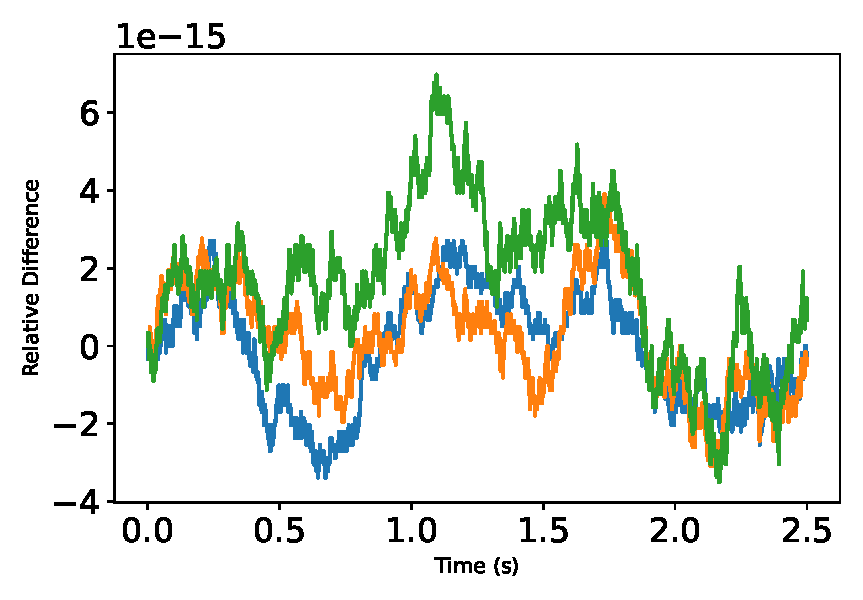
\includegraphics[width=0.8\textwidth]{AutoTeX/ChangeInOrbitalAngularMomentumNoGravity}}
	\caption{Change In Orbital Angular Momentum No Gravity}
	\label{fig:ChangeInOrbitalAngularMomentumNoGravity}
\end{figure}
\begin{figure}[htbp]
	\centerline{
		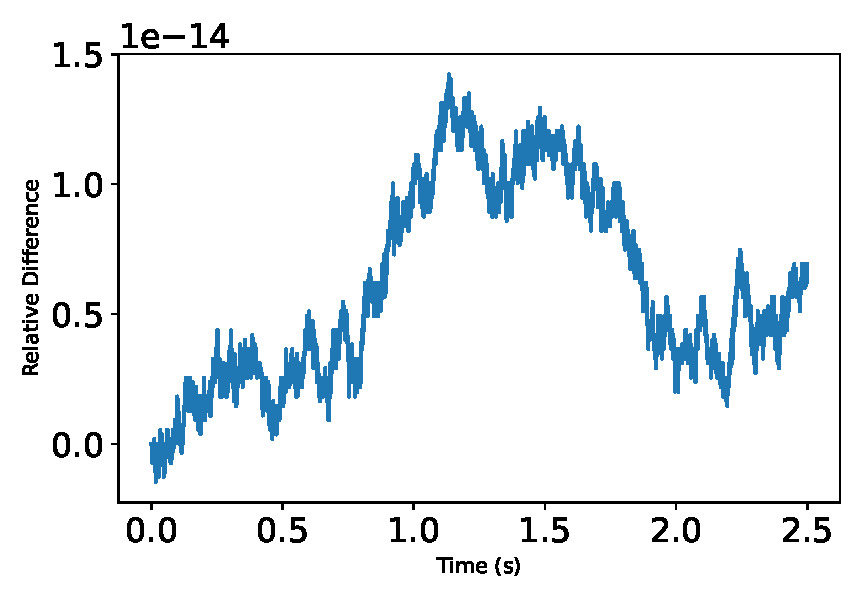
\includegraphics[width=0.8\textwidth]{AutoTeX/ChangeInOrbitalEnergyNoGravity}}
	\caption{Change In Orbital Energy No Gravity}
	\label{fig:ChangeInOrbitalEnergyNoGravity}
\end{figure}
\begin{figure}[htbp]
	\centerline{
		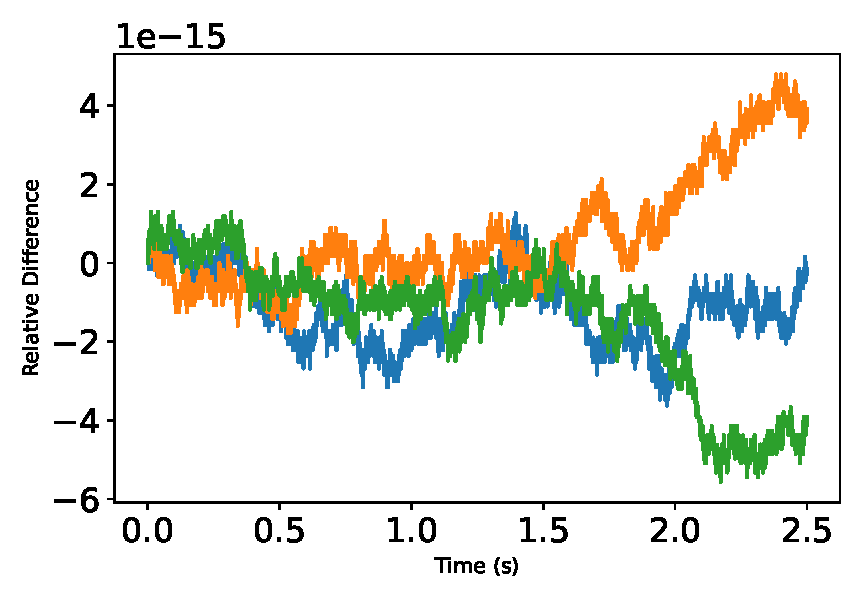
\includegraphics[width=0.8\textwidth]{AutoTeX/ChangeInRotationalAngularMomentumNoGravity}}
	\caption{Change In Rotational Angular Momentum No Gravity}
	\label{fig:ChangeInRotationalAngularMomentumNoGravity}
\end{figure}
\begin{figure}[htbp]
	\centerline{
		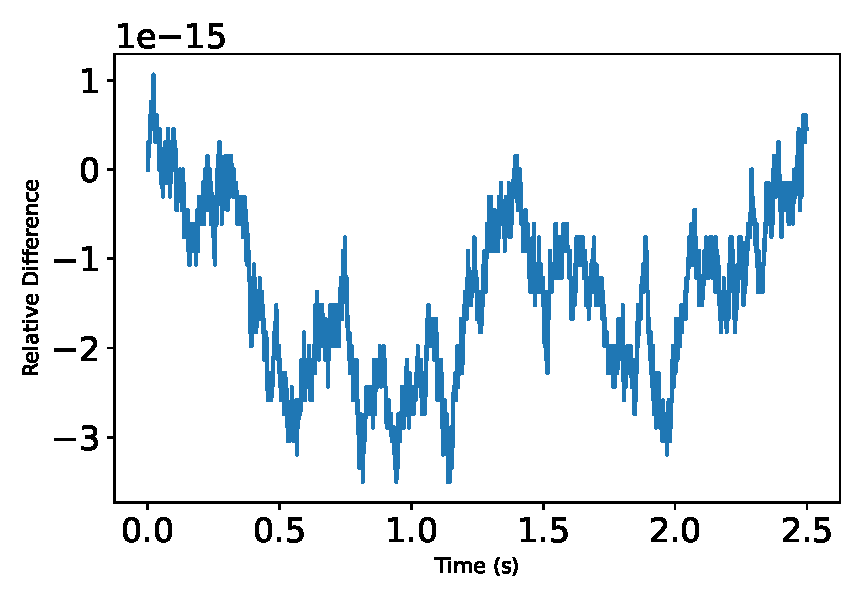
\includegraphics[width=0.8\textwidth]{AutoTeX/ChangeInRotationalEnergyNoGravity}}
	\caption{Change In Rotational Energy No Gravity}
	\label{fig:ChangeInRotationalEnergyNoGravity}
\end{figure}

\clearpage

\subsection{Damping with no gravity scenario}
\begin{figure}[htbp]
	\centerline{
		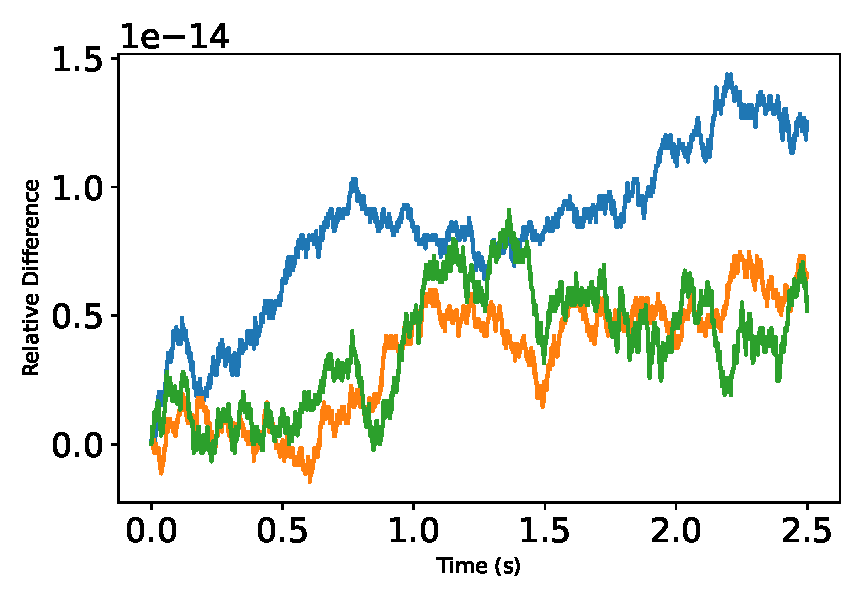
\includegraphics[width=0.8\textwidth]{AutoTeX/ChangeInOrbitalAngularMomentumDamping}}
	\caption{Change In Orbital Angular Momentum Damping}
	\label{fig:ChangeInOrbitalAngularMomentumNoGravityDamping}
\end{figure}
\begin{figure}[htbp]
	\centerline{
		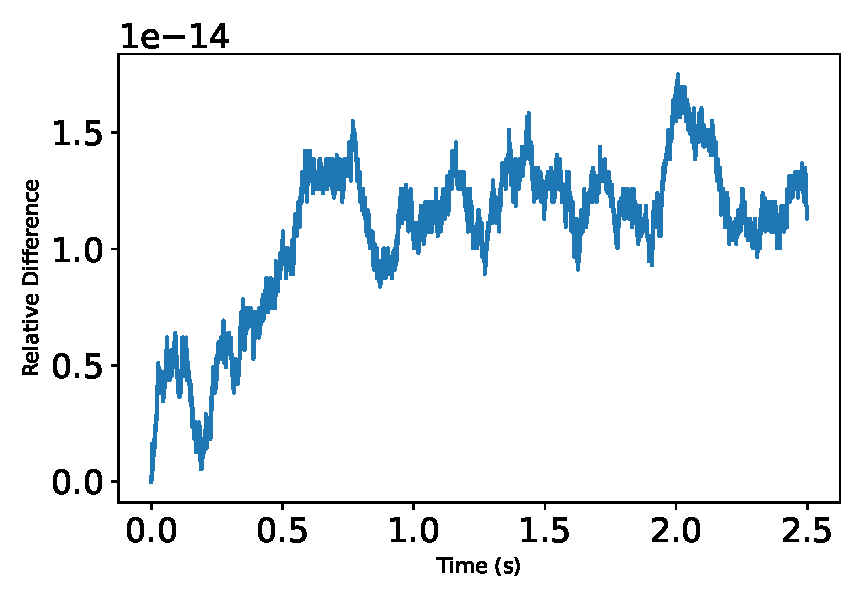
\includegraphics[width=0.8\textwidth]{AutoTeX/ChangeInOrbitalEnergyDamping}}
	\caption{Change In Orbital Energy Damping}
	\label{fig:ChangeInOrbitalEnergyDamping}
\end{figure}
\begin{figure}[htbp]
	\centerline{
		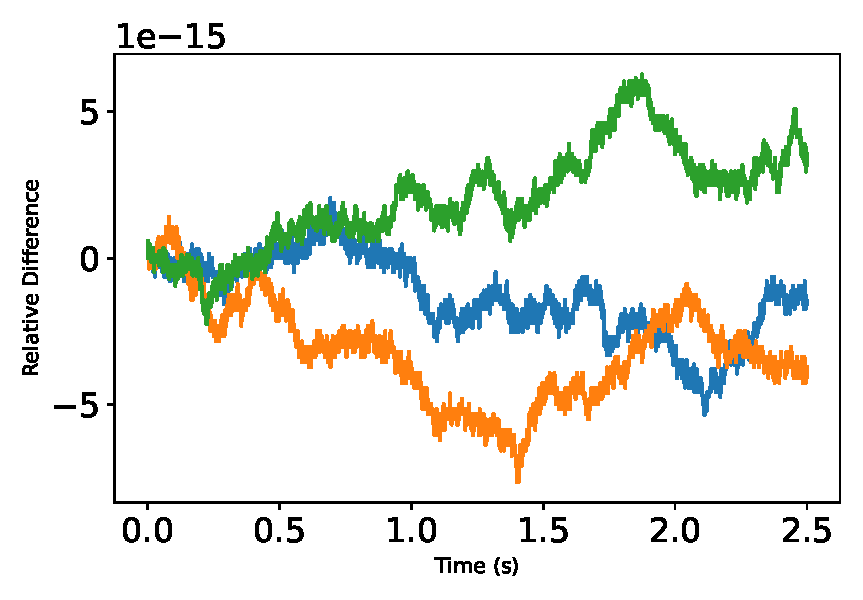
\includegraphics[width=0.8\textwidth]{AutoTeX/ChangeInRotationalAngularMomentumDamping}}
	\caption{Change In Rotational Angular Momentum Damping}
	\label{fig:ChangeInRotationalAngularMomentumDamping}
\end{figure}
\clearpage
